\documentclass[12pt,twoside]{reedthesis}
\usepackage{graphicx,latexsym} 
\usepackage{amssymb,amsthm,amsmath}
\usepackage{longtable,booktabs,setspace} 
\usepackage{url}
\usepackage{natbib}
\usepackage{algorithm}
\usepackage{algorithmic}

\title{My Final College Paper}
\author{Ivan A. Malison}
\date{April 2012}
\division{Mathematics and Natural Sciences}
\advisor{James D. Fix}

\department{Mathematics}


\setlength{\parskip}{0pt}
\begin{document}

  \maketitle
  \frontmatter 
  \pagestyle{empty}

  \chapter*{Acknowledgements}

% The preface is optional
% To remove it, comment it out or delete it.
    \chapter*{Preface}

    \tableofcontents

    \chapter*{Abstract}
	
	\chapter*{Dedication}

  \mainmatter 
  \pagestyle{fancyplain}

    \chapter*{Introduction}
         \addcontentsline{toc}{chapter}{Introduction}
	\chaptermark{Introduction}
	\markboth{Introduction}{Introduction}

        %%Open CL architecture%%
\chapter{GPU Computing}
\section{Background}
\section{OpenCL}

\chapter{Matrix Multiplication}
\chapter{Single Source Shortest Paths}
\section{Background}
\section{Sequential Algorithms}
\subsection{Dijkstra's Algorithm}
\subsection{Bellman Ford}


\chapter{Prefix Sums}
Let $a = a_0, a_1, a_2, \ldots a_{n-1}$ be a finite sequence of $n$
numbers.  The prefix sum of $a$, is a sequence $b = b_0, b_1, b_2,
\ldots b_{n-1}$ where $b_i = \sum_{a = 0}^i a_i$.

%%insert a trivial example%%

%%talk about why prefix sums are useful???%%

\vspace{1pc}

Note that the following equivalence holds for all $i > 0$:

$$
b_i = b_{i-1} + a_i
$$

The preceeding equation strongly suggests a natural algorithm to
compute prefix sums on a sequential computer. The first element of
the output sequence serves as a kind of base case; since there is
only one element in our sum, no operations need to be performed, and so we can simply copy the first element of the input sequence to the first element of the output sequence.  To compute the remaining values of the output sequence we iterate through the input sequence starting at the second element.  As the equivalence above suggests, we compute the corresponding value in the output sequence by adding the value of the input sequence ($a_i$), to the value we just computed ($b_{i-1}$). The following is a pseudocode implementation of the aforementioned algorithm, where both the input and output sequences are stored in memory as arrays (the reader should note that other data structures like linked lists are amenable to the same algorithm with only trivial modifications).

\begin{algorithm}
\caption{A sequential implementation of the prefix sum operation.}
\begin{algorithmic}
\STATE output[0] $\leftarrow$ input[0]
\FOR{$i = 1 \to  n-1$}
\STATE output[$i$] $\leftarrow$ output[i-1] + input[i] 
\ENDFOR
\end{algorithmic}
\end{algorithm}

It is easy to see that it is impossible to come up with an algorithm
that performs better than this one in any reasonable model of
sequential computation. There is simply no way to circumvent the $n-1$
addition operations performed in this algorithm as the final
value of our output sequence is the sum of $n$ values (which cannot be
computed with fewer than $n-1$ additions operations). Similarly, each
item in the input sequence must be read, and a value must be stored to
each location in the output sequence.  As we have accounted for every operation performed in the algorithm, we conclude that it is optimal within the model of computation we are using.

The reader should note that the prefix sum operation can be
generalized to use any binary associative operator in the place of
addition. For example, it is possible to compute the prefix minimums
of a sequence, since the operation of minimizing two numbers is associative.

Given that the sequential implementation of prefix sums is so natural,
it is tempting to conclude that something about the operation is
inherently sequential. After all, there is no getting around the fact
that to calculate the $i$th value of the output sequence
$i-1$ operations must be preformed. Surprisingly, it turns out that
there are a family of parallel algorithms that compute prefix sums in
an amount of time that is asymtotically than the amount of
time taken by the sequential algorithm.


\section{Parallel Prefix Sums}
%%Word about PRAM architecture%%
%%CREW%%

The following section culminates in the description of an alogorithm
that efficiently computes the prefix sums of an arbitrary sequence on
a PRAM architecture with any number of processors.
%% intro stuff %%

For the time being, we make the simplifying assumption that the number of processors available to us, $p$, is half the number of elements in our sequence $n$. Furthermore, we assume that $p=n=2^k$ for some integer value of $k$.

%%calculating the simple sum of a sequence%%
\vspace{1pc}
\subsection{Parallel Left Fold}
We begin by describing a parallel algorithm for the left fold operation, which is a close relative of prefix sums/scan operation.

Like scan, parallel-left-fold takes a sequence $a = a_0, a_1, a_2, \ldots a_n$ together with a binary associative operator, $\oplus$. The output of this operation is the single value

$$a_0 \oplus a_1 \oplus a_2 \oplus \ldots \oplus a_{n-1}$$

When the binary operation provided is conventional addition, parallel-left-fold produces the total sum of the input sequence. One might say that parallel-left-fold is a simplified version of scan where only the last value of the sequence is computed.
\vspace{.5pc}

Consider that for any associative binary operator $\oplus$:
\begin{equation}
a_0 \oplus a_1 \oplus a_2 \oplus \ldots \oplus a_{n-1} = (a_0 \oplus a_1) \oplus (a_2 \oplus a_3) \oplus \ldots \oplus (a_{n-2} \oplus a_{n-1}) \label{assocident}
\end{equation}

This simple rewrite suggests an equivalence between the sequences $a$ and $a' = (a_0 \oplus a_1), (a_2 \oplus a_3), \ldots, (a_{n-2} \oplus a_{n-1})$, in terms of parallel-left-fold.

$$
\mbox{parallel-left-fold}(a, \oplus) = 
a_0 \oplus a_1 \oplus a_2 \oplus \ldots \oplus a_{n-1} =
$$
\begin{equation}
(a_0 \oplus a_1) \oplus (a_2 \oplus a_3) \oplus \ldots \oplus (a_{n-2} \oplus a_{n-1}) = 
\mbox{parallel-left-fold}(a', \oplus)
\label{pfoldi}
\end{equation}

Note that while the way we described $a'$ depends on the assumption that $n$ is even, the equivalence above also holds for $n$ odd when we set the final element of $a'$ to be $a_{n-1}$.
\vspace{1pc}

The equivalence (\ref{pfoldi}) implies that the problem of calculating parallel-left-fold on a sequence of length $|a| = n$ can be reduced to the problems of calculating the sequence $a'$ from $a$, and calculating parallel-left-fold of a sequence of size $|a'| = \lceil \frac{n}{2} \rceil$. This observation can be transformed in to a precise statement about the runtime of parallel-left-fold:

\begin{equation}
T(n) = T(n/2) + A(n) 
\label{rr}
\end{equation}

Where $T(n)$ is the running time of parallel-left fold and $A(n)$ is
the amount of time it takes to calculate the sequence $a'$ from $a$. 

Note that we can apply this identity to itself to produce another
reduction of our problem, $T(n) = T(n/4) + A(n/2) + A(n)$. The idea
behind parallel-left-fold is to recursively apply this reduction until
the sequence we are left with a sequence of length one. The only term
in this sequence will be the value of parallel-left-fold of the
original sequence. This algorithm can be represented visually in the
form of a balanced binary tree.

\begin{figure}[h]
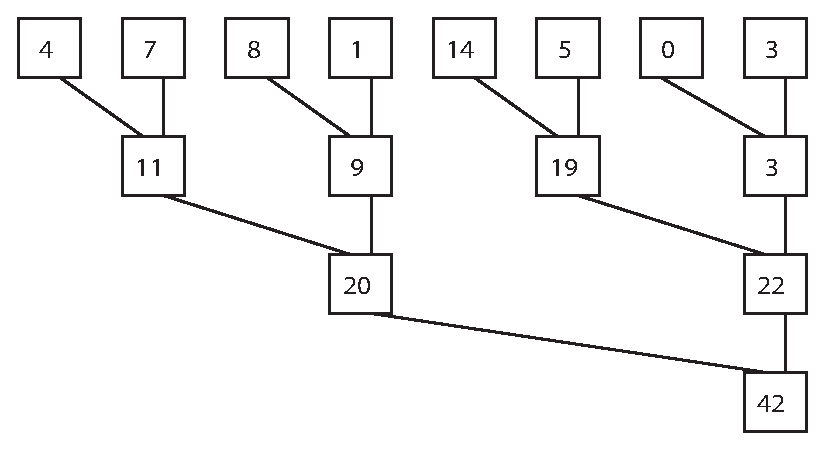
\includegraphics{parallel-left-fold-tree.pdf}
\caption{An illustration of the successive reduction of
  parallel-left-fold where $\oplus$ is set to be addition.}
\end{figure}
\vspace{1pc}

This figure is drawn with the parents right aligned to indicate that
the result of the addition ends up overwriting the slot originally
occupied by the second summand. The bottom-most value in each column
of the graphical representation will be the final value stored in the
temporary array that stores intermediate sums.

An explicit procedure to determine which processor performs each
$\oplus$ operation must be devised to complete this implementation of
parallel-left-fold. Note that each level in this tree represents a reduction of the original input
sequence. Since we have a balanced binary tree, the number of nodes at
the $j$th level (starting at 0) of the tree is  $\lceil \frac{n}{2^j}
\rceil$. Thus we need $\lceil \frac{n}{2^i}\rceil$ processors to
perform the $i$th (starting at 1) reduction of our sequence.
Note that there are exactly $\lceil \frac{p}{2^j} \rceil = \lceil
\frac{n}{2^{j+1}} \rceil$ numbers $l$ in the range 0 to $p-1$ for
which $(l \mod 2^j = 0)$. This means that the modulus operator can be
used, together with a variable that is multiplied by two in each
iteration to select which processors will be active. Since all $p$ of
our processors must be active in the first round, we will initialize
this variable to the value of 1. Note that this value also corresponds
to the distance between the values that each processor will add in any
particular reduction. The following pseudo-code describes the rest of
the details of the implementation.

\begin{algorithm}[h!]
\caption{parallel-left-fold where $p = n/2$ and $n=2^k$}
\begin{algorithmic}
\STATE values[pid] $\leftarrow$ input[$2\cdot \mbox{pid}$] $\oplus$ input[$2\cdot \mbox{pid} +1$]
\STATE stride $\leftarrow$ 1
\WHILE{$\mbox{pid} \mod \frac{n}{\mbox{stride}} = 0$ and $\mbox{stride} < n$}
\STATE values[pid] $\leftarrow$ values[pid] $\oplus$ values[pid $+$ stride] 
\STATE stride $\leftarrow$ stride$\cdot 2$
\ENDWHILE
\RETURN values[0]
\end{algorithmic}
\end{algorithm}

%%Since each of the computations a particular depth in the tree above are computed in lock step, the height of the tree is the running time of parallel-left fold.  Since the tree above is a balanced binary tree with $n$ leaves it has height $\lceil log_2 n \rceil$. This result can also be obtained by solving the recurrence relation (\ref{rr}) with the base case $T(1) = 0$.%%

\vspace{3pc}
\subsection{A First Attempt}

In computing parallel-left-fold in the manner described above, some of the partial sums that constitute the output of parallel-prefix-sums are computed.

\begin{figure}[h]
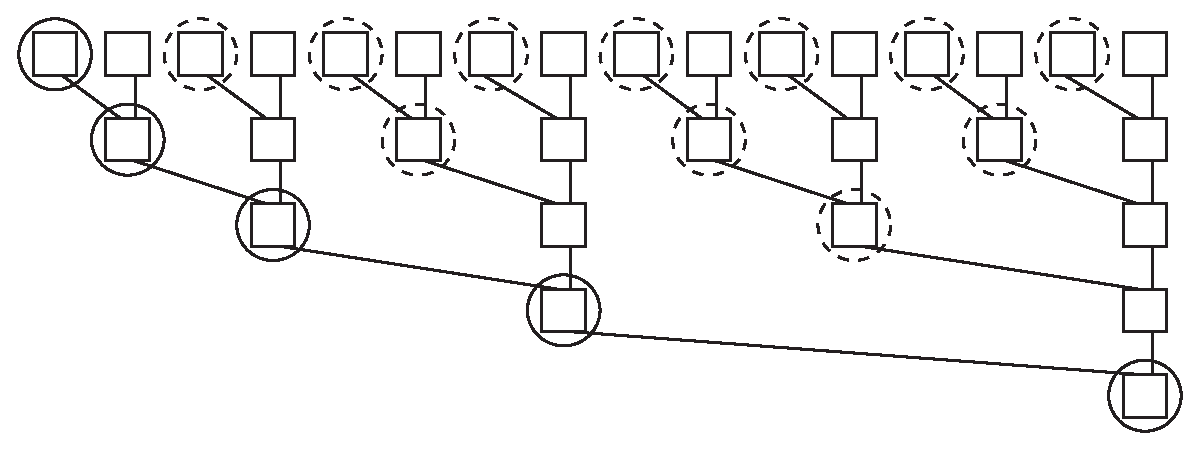
\includegraphics[scale = .75]{correctsums.pdf}
\caption{Each node in the tree that represents the final in a slot of the temporary array is circled. A solid line indicates that the value is correct, while a dashed line indicates that the value is incorrect.}
\end{figure}
\vspace{1pc}

Specifically, all the partial sums that are placed at output indices $2^a-1$ for positive integers $a$ are correct. The other sums that are computed as intermediaries to the final sum are incomplete in the sense that they are only correct prefix sums for some continuous subsequence of the input sequence. In general, the sum in the temporary array at the $i$th index after the execution of parallel-left fold is the sum of the subsequence ending at $a_i$, and including $2^j$ terms\footnote{$a_{i-(2^j-1)}, a_{i-(2^j-1)+1}, \ldots a_i$}, where $j$ is the final round in which that value was modified.
\begin{proof}
What we will prove is that at the value at any array index $i$ that is active during the $j$th reduction is the subsequence of length $2^j$ ending at the $i$th value of the input sequence. This directly implies that the value that remains after the execution of the entire algorithm will be the value after the final reduction in which that value was changed.

We prove this claim by induction on $j$. When $j=0$ the values in the temporary array are just the values of the input sequence. Since $j=0$, $2^j = 1$, and indeed, the values of the input sequence are the trivial sums of length one, 

Suppose that the node $i$  is active during the $j+1$th reduction step. Then by our induction assumption, its value just before that reduction step is executed is the correct subsequence of length $2^j$. Similarly, the array value that is to be added to our value was also active at the $j$th reduction
\footnote{The value at the $z$th array index is active in the $j+1$th round when $z+1 \mod 2^{j+1} = 0$ and. Thus $z - 2^j + 1 = 0 \mod 2^j$, since both $z+1$ and $2^j = 0 \mod 2^j$.}
, and so its subsequence is also the correct subsequence of length $2^j$. As noted in the previous section, the distance between terms added in the $j$th reduction is always $2^j$, which means that these two sequences have no overlapping terms, and no missing terms in between them. By the associativity of the operator that is being used, the value that results from applying $\oplus$ to these two terms is the subsequence ending at the rightmost index of length $2^j + 2^j = 2 \cdot 2^j = 2^{j+1}$.
\end{proof}

With this fact, one can formally determine which 


\begin{algorithm}[h!]
\caption{parallel-prefix-sums where $p = n/2$ and $n=2^k$}
\begin{algorithmic}
\STATE output[pid] $\leftarrow$ input[$2\cdot \mbox{pid}$] $\oplus$
\STATE stride $\leftarrow$ 1
\WHILE{$\mbox{pid} \mod \frac{n}{\mbox{stride}} = 0$ and $\mbox{stride} < n$}
\STATE values[pid] $\leftarrow$ values[pid] $\oplus$ values[pid $+$ stride] 
\STATE stride $\leftarrow$ stride$\cdot 2$
\ENDWHILE
\RETURN

\STATE myitem $\leftarrow$ pid $\cdot 2$ 
\STATE segmentsize $= n/2$
\WHILE{stride $> 0$}
\IF{myitem $\mod$ segmentsize $= 0$ and pid $!=$ 0}
\STATE values[myitem -1 + segmentsize/2] += values[myitem-1]
\ENDIF
\STATE segmentsize = segmentsize/2

\ENDWHILE
\end{algorithmic}
\end{algorithm}
	
\chapter*{Conclusion}
         \addcontentsline{toc}{chapter}{Conclusion}
	\chaptermark{Conclusion}
	\markboth{Conclusion}{Conclusion}
	\setcounter{chapter}{4}
	\setcounter{section}{0}
	

    \appendix
      \chapter{The First Appendix}



  \backmatter 

    \bibliographystyle{bsts/mla-good} % there are a variety of styles available; 
    \nocite{*}
    \bibliography{thesis}
\end{document}
